\chapter{PLUME laboratory testing}
\label{chap:labTests}

  The chapter~\ref{chap:vxd} has described the \gls{PLUME} project with the different prototypes that were built. 
  Since the version-1 of \gls{PLUME}, the detector is more complicated due to the six sensors on a module that have to be synchronised and the flex-cable which has a lot of metal traces to pilot and read the senors.
  Before to perform test in real conditions at CERN or at DESY, the device has to be validated and characterised first in the lab.
  This chapter is introducing the different steps from the assembly procedure performed at Strasbourg (for the module) and Bristol (for a complete ladder), to the final tests with a radiation source, and include electrical functionality tests.

  %The \gls{PLUME} ladders are complex detectors and the last prototype was designed to optimise the material budget, by decreasing the width of the flex-cable and the metal traces.
  %Before to perform test in real conditions, the device has to be validated and characterised first in the lab.
  %This chapter is introducing the different steps from the assembly procedure performed at Strasbourg and Bristol, the electrical functionality checks to the tests with a radiation source,
 
 \minitoc
  
  %\begin{itemize}
  %  \item Describe bench
  %  \item Describe control of a sensor
  %  \item Describe output of Mi-26
  %\end{itemize}

\section{Visual inspection}

  The ladders are built in two steps. 
  Firstly, two independent modules are mounted at Strasbourg, then tested at DESY, to be then shipped at Bristol were the modules are glued together on a \gls{SiC}.
  The assembly procedure are introduced here and then the visual inspection is described.

  \subsection{Module and ladder assembly}

    \subsubsection{Module assembly}
    \label{subsec:modAssembly}

      The module assembly is performed at the IPHC by the microelectronics group and is done in three steps.
      First of all, the passive components are soldered onto a flex-cable.
      Then an epoxy layer with a thickness of $300 \mu\text{m}$ is glued under the connector side.
      This layer is used to reinforce the flex-cable on this non sensitive part due to the force applied by pulling and pushing the jumper cable.
      The module is then placed on a metal jig to insure its flatness thanks to a vacuum suction.
      The next step consists to glue the six sensors onto the flex.
      As they are thin and fragile pieces, the manipulation is done thanks to a vacuum sucker.
      Few drops of glue are dispensed on the flex and then the sensors are gently pressed one by one on top of it to be glued.
      The glue is then cured in a oven.
      The positioning of the sensors was used to be done manually, but a programmable robot is now in charge of it.
      The maximum mismatch alignment reaches $20 \mu\text{m}$. 
      The gluing procedure is definitive. 
      If a sensor is not working properly, it can't be removed and replaced by a new one because of the fragile flex-cable.
      On the worse case, a new sensor can be glued on top of it, but this procedure will increase the material budget.
      In order to avoid this situation, the sensors are probe tested at IK in Frankfort before the module assembly to select only the good ones.
      The final step consists to solder the 540 wire-bonds (a single MIMOSA-26 requires 90 wire-bonds) thanks to a semi-automatic machine.
      The wire-bonds can be protected by applying a glob top epoxy.
      It has the advantage to offer a protection against moisture ore contaminants, an electrically insulation and prohibits their movement during other manipulations. 
      Nevertheless, it increases the material budget on this area and if there is an electrical problem, the wire-bonds can't be disconnected.
      To test the module, it is transferred onto a plastic sole that has alignment pins.
      This sole is completed with a plastic cover to protect completely the module during shipping.

      %Control of absolute position about 10 $\mu\text{m}$.
      %Distance between edge of pixel of neighbouring sensors about $500 \mu\text{m}$.
      %Mismatch about $20 \mu\text{m}$.

      %The next step is to sold the wire-bonds (90 for a single Mi26) : semi-automatic machine
      %Modules are then transferred onto a plastic sole for testing and or shipping.

    \subsubsection{Ladder assembly}

    The ladder assembly is performed by the Bristol team.
    It consists to group two module together on a spacer (\gls{SiC}) and a bate (an aluminum plate).
    The operation is done entirely by hands.
    Each module are placed on a separate jig thanks to alignment pins to ensure the positioning.
    The sensor side is facing the jig to have an access to the rear of the module for gluing.
    Then, the foam is placed on one module below the sensors, while the bate is glued below the connector with and overlaps the foam.
    The second module receive some glue on the backside before the jigs are assembled together.
    The glue is then cured for one day.
    The amount of glue needed for the assembly was studied carefully. 
    Indeed, the surface of the foam is not regular, so if not enough glue is used, the foam will not be glued on the module.
    On the other hand, using too much glue might stick the jigs together.
    When the ladder is finally ready, it is placed in an aluminum box used for shipping but also testing.
   
  \begin{figure}[!h]
    \centering
    \begin{subfigure}[t]{0.4\textwidth}
        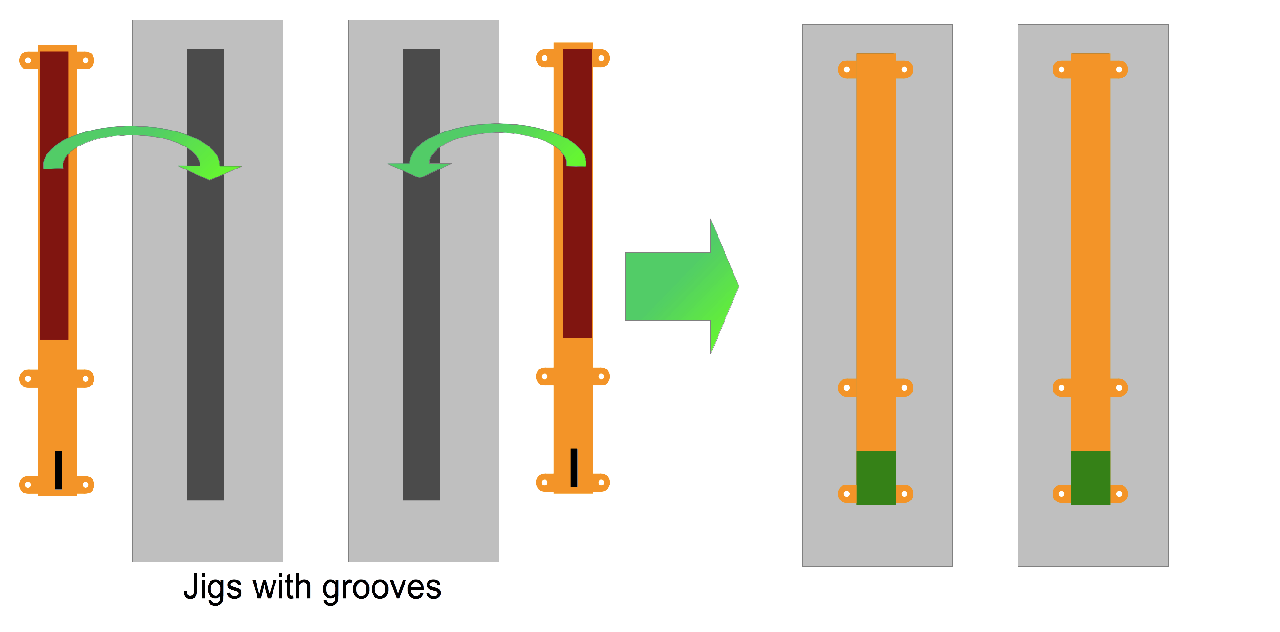
\includegraphics[width=1.2\textwidth]{Pictures/labTests/plumeLadderAssembly_step1.png}
        \caption{}
        \label{fig:ladderAssemblyStep1}
    \end{subfigure}
    \qquad
     %add desired spacing between images, e. g. ~, \quad, \qquad, \hfill etc. 
      %(or a blank line to force the subfigure onto a new line)
    \begin{subfigure}[t]{0.4\textwidth}
        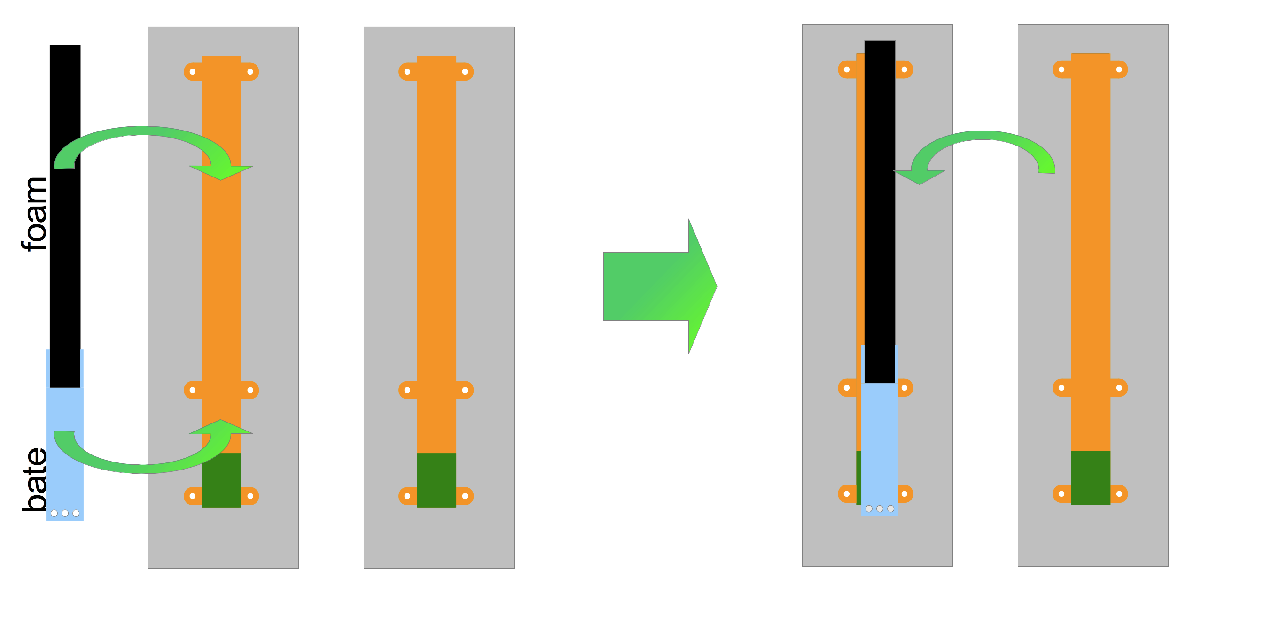
\includegraphics[width=1.2\textwidth]{Pictures/labTests/plumeLadderAssembly_step2.png}
        \caption{}
        \label{fig:ladderAssemblyStep2}
    \end{subfigure}
    \caption{Drawing of the ladder assembly. The modules are first placed on the jigs, sensors facing the grooves~\ref{fig:ladderAssemblyStep1}, then the foam and the bate are glued between the two modules~\ref{fig:ladderAssemblyStep2}.}\label{fig:ladderAssembly}
    \end{figure}    

  \subsection{Visual inspections}

  As explain in subsection~\ref{subsec:modAssembly}, the sensors positioning was performed firstly manually and later was switched to an automatic procedure.
  To tune properly the robot which is in charge of the sensor positioning, the microelectronic group needs a position feedback.
  The modules are then inspected under a microscope to measure the gap between two sensors, and their position relatively to each other.
  The distance between the last pixel of a sensor to the neighboring one should be less than $500 \mu\text{m}$.
  The mismatch of the robot is about $20\mu\text{m}$. 
  The figure~\ref{fig:visAlign} is a picture taken with a microscope showing the relative position of two sensors on the bottom of the matrix.
  %A visual inspection of the position,  as well as any problem on the matrix, as a crack, as well as a check of the wire-bonds have to be done before any electrical validation.
  The gap between the two edges is approximately ... \todo{Measure gap between the sensors}. 
  
  \begin{figure}
    \centering
    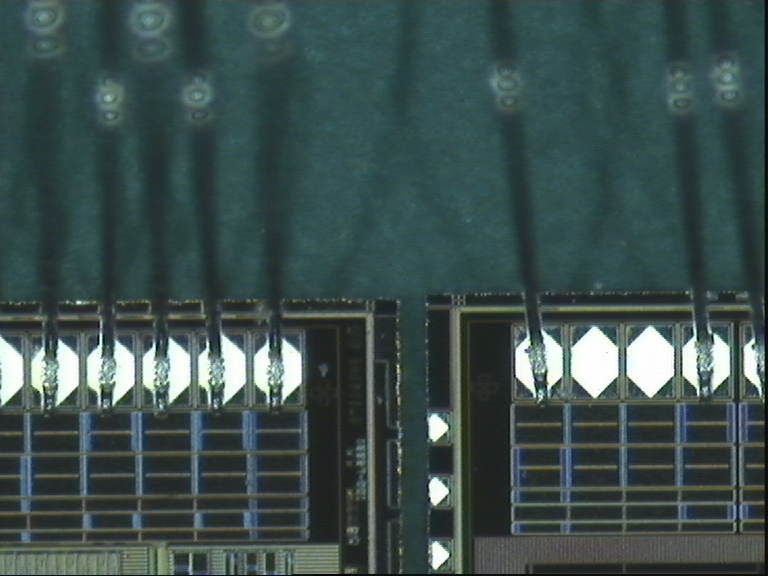
\includegraphics[width=0.6\textwidth]{Pictures/labTests/alignment_sensors.jpg}
    \caption{Visualisation of the alignment}
    \label{fig:visAlign}
  \end{figure}
  
  The visual inspection is also needed to check if the wire-bonds is correct, to look for a crack on a sensor and to verify that the module survive the shipping between Strasbourg and DESY.
  The modules are very sensitive objects that should be handle carefully.

  %\begin{itemize}
  %  \item Check positioning matrix defect (crack)
  %  \item Check wire bonds
  %  \item Check alignment
  %\end{itemize}

  \begin{figure}
    \centering
    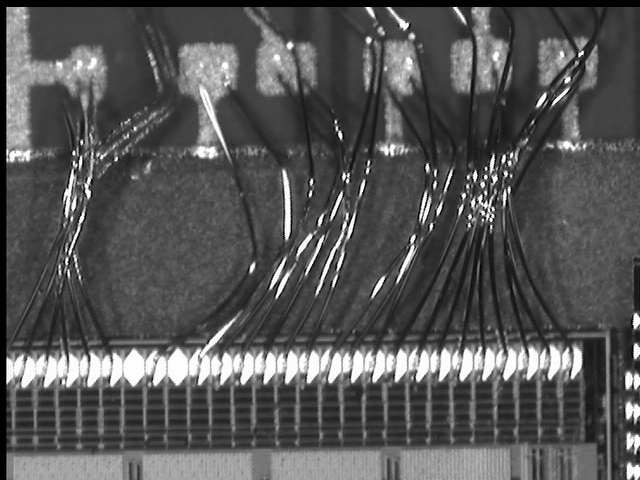
\includegraphics[width=0.6\textwidth]{Pictures/labTests/crash_bonds.jpg}
    \caption{Wire bonds damaged }
  \end{figure}

\section{Electrical validation}

  The electrical validation of a \gls{PLUME} module or ladder is done in two steps.
  The first one consists to check that all the system controlling and powering the module is working. 
  Then, the module is connected and its consumption, as well as the communication are checked.

  \subsection{Auxiliary board}

  On one edge of the module, a ??? connector is used to power the sensors, but also to pilot them and to transfer the data to the outside world.
  A jumper cable is connected between the module and an auxiliary board.
  This board is connected to a power supply board which is providing the nominal voltages needed by the module.
  The auxiliary board is also connected to a computer for the slow control.
  Two RJ45 are in charge to provide the JTAG registers, as well as the start, the reset signal and in a case of a complete ladder an external clock.

  For the test procedure, but also for the acquisition, the PLUME module is connected to an acquisition board, via a jumper cable.
  This board is in charge to distribute the power supplies, the control signals and the data output.
  A power supply board is providing the $\text{V}_{dd_d}$ and $\text{V}_{dd_a}$, the $\text{V}_{CC}$ and 5 V.
  The $\text{V}_{dd_d}$ and $\text{V}_{dd_a}$ are tunable thanks to two potentiometers, while $\text{V}_{CC}$ is fixed.

  A PLUME module is connected to an auxiliary board via a jumper cable in order to be operated.
  This auxiliary board is providing the power supply and the slow control to the ladder and give then an access to the sensors' output.
  Two RJ45 inputs are providing the slow control, the reset and start signal and has the possibility to provide an external clock, used only when two modules are working together to make sure that they are synchronised.
  A power supply board, connected to the auxiliary board, is providing the digital and analog voltage, plus 

  An auxiliary board is in charge to power a PLUME module and to send the slow control to pilot each sensor. 
  If only one module is tested, an oscillator is providing the 80 MHz clock.

  Sixteen pads are used to read the response of the six sensors and the clock and marker of the sensor number 6.
  It also has an output connection to check the response of each sensor with an oscilloscope, as well as for the acquisition.
  It is in charge to provide the 80 MHz clock, via oscillator or via an external input. 

  \begin{itemize}
    \item Generate the 80 MHz for the 6 Mi 26 by oscillator on board or by an external input.
    \item Bufferisation of the Digital signals sent to the chips (JTAG and control signals) and the digital signal provide by the 6 Mi26 to the DAQ in LVDS .
    \item Regulators for the power supply of the sensors.
    \item Power pulsing
    \item Current measurement
    \item test point for the DAC characterisation
  \end{itemize}

  The consumption of the auxiliary board and the power board is around $380 \mu\text{m}$.
  Then, the auxiliary board is checked to be sure that the signal route is working properly.
  Two RJ45 are connected to the aux board. One is dedicated to the slow control (or JTAG) and the second one is dedicate to the control, clock, start and reset signal.

  \begin{figure}
   % \centering
    \missingfigure{Sketch of Auxiliary board}
  \end{figure}

  Explanation of Vdd\_d, Vdd\_A, Vclp.
  \begin{itemize}
    \item Consumptions
    \item Explanation of different voltages applied:
    \begin{itemize}
      \item $\text{V}_{dd_D} = 3.3V $
      \item $\text{V}_{dd_A} = 3.3V $
      \item $\text{V}_{clp} = 2.1V $
    \end{itemize}
    \item JTAG control explanations
  \end{itemize}

  \subsection{Smoke test}

  After the connections were controlled and before to connect the module to the bench, the different voltages has to be set.

  \begin{itemize}
    \item Check consumption
    \item Check JTAG control
    \item Check Output
  \end{itemize}

  \subsection{Mimosa-26 output}

  An inspection of the output with an oscilloscope is performed to check the slow control and to estimate the response of the sensor.
  The information provided by a sensor is contained in four output lines.
  On a PLUME ladder, all the sensors are synchronised, so only the clock and marker from the last sensor is provided.
  The clock is always present and its rate depends on the clock register. 
  In a normal mode, the rate is 80 MHz.
  The second output is the marker. 
  It is available in all modes and its signal last during 4 clock cycles (starting at the rising edge) and is used to know the beginning of the data transmission.
  The data itself are divided on two output Data0 and Data1. 
  It contains the \textit{header} and \textit{tail} that allows to detect the beginning and the end of a data transmission.
  The signal is composed of $2 \times 16$ bits and its configurable via the \gls{JTAG}.
  Then, 16 more bits are indicating the \textit{frame counter}.
  It corresponds to the number of frame since the chip was reset.
  After that, the \textit{data length} provides an information on the length of the useful data.
  The useful data \textit{state} and \textit{status}

\section{Noise measurements}

  \begin{itemize} 
    \item Describe steps
    \item Describe analysis
    \item FHR with normal acquisition
  \end{itemize}

  \begin{figure}
    \centering
    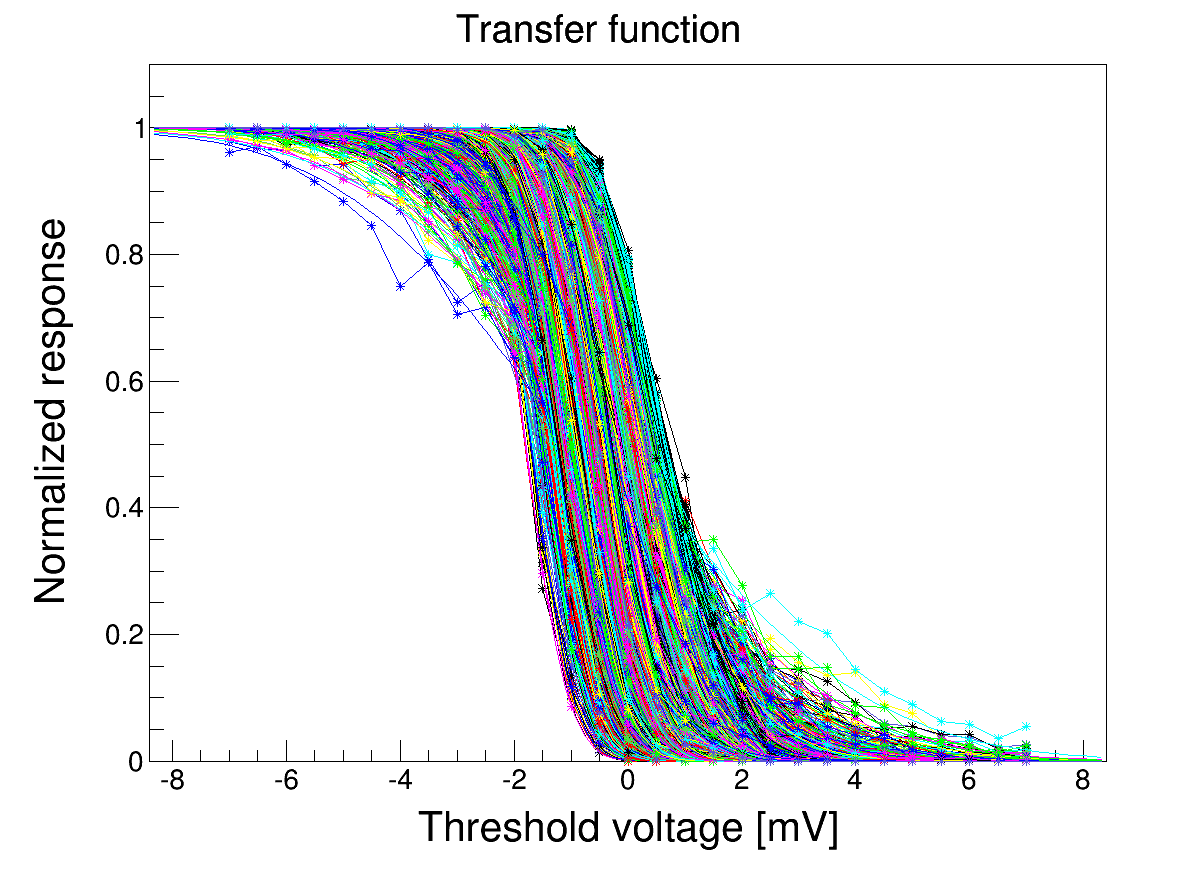
\includegraphics[width=0.6\textwidth]{Pictures/labTests/transfer_B.png}
    \caption{Pixels response of a threshold scan around the middle-point of discriminators for a sub-matrix.}
  \end{figure}

  \begin{figure}
    \centering
    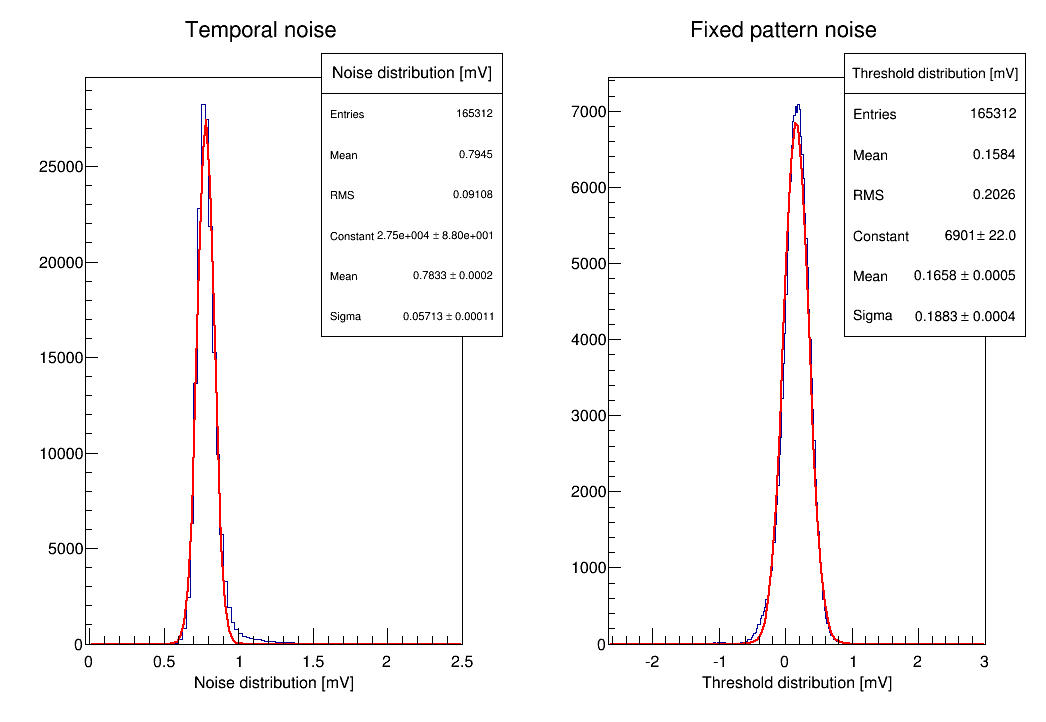
\includegraphics[width=0.8\textwidth]{Pictures/labTests/noise_A.png}
    \caption{TN and FPN}
  \end{figure}
  
  \begin{figure}
    \centering
    
\includegraphics[width=0.6\textwidth]{Pictures/labTests/8sigma_10kEvents_noSource}
    \caption{Accumulation of 10k events at a thresholds of 5 times the noise acquired in the dark.}
  \end{figure}

  \begin{figure}
    \centering
    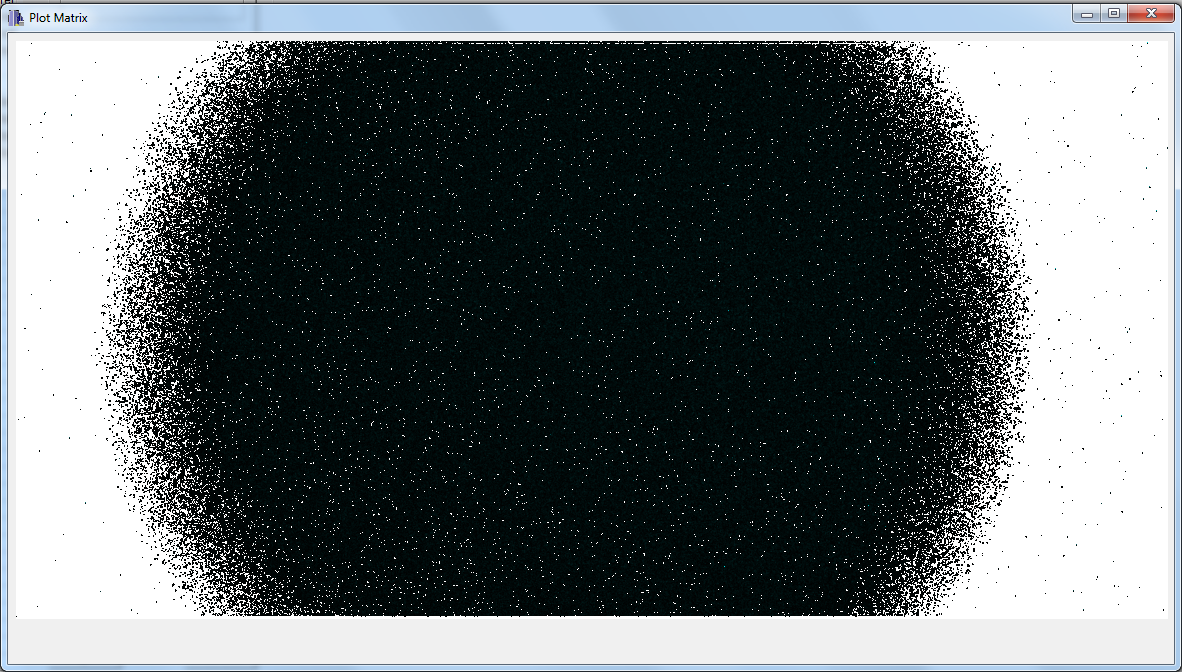
\includegraphics[width=0.6\textwidth]{Pictures/labTests/10kEvents_Fe55_cut5sigma.png}
    \caption{Accumulation of 10k events at a thresholds of 5 times the noise with Fe55 radiation source.}
  \end{figure}

  \begin{figure}
    %\centering
    \missingfigure{FHR = f(Threshold)}
  \end{figure}

\section{Cluster}

  \begin{figure}
    %\centering
    \missingfigure{Cluster shape}
  \end{figure}
